\chapter{Gestion du projet}
\section{Organisation du projet}
Dès le départ, nous avons décider de travailler avec git, plus précisement 
en utilisant le site \url{https://github.com}. Nous avons donc créé une organisation afin de séparer les différents dépots. Nous en avons définis 2, mais les membres de l'organisation étaient libres d'en ajouté d'autres.
\begin{itemize}
    \item crapauduc.  Ce dépôt est le dépot principal où les notebooks des modèles sont déposés, nous y avons aussi placé les rapports des anciens étudiants afin d'y avoir un accès rapide. Nous y avons aussi déposé un subset d'image d'environ 0.5 Gib permettant le fine tuning.
    \item utils. Ce dépôt contient des scripts faisant des transformormations ou des analyses sur les données. Nous y avons par exemple un script qui permet de convertir les annotations de csv à COCO.
\end{itemize}

De plus, nous avons créer un compte google ayant le doux nom de \verb|student GML| afin d'avoir un espace google drive de 15 GiB pour stocker les données ainsi qu'une intégration facilitée dans le service \url{colab.research.google.com/} de Google. Nous croyions être prêts.


\section{Gestion du temps de travail}
Dès le départ, nous avons décider de travailler à distance afin de dédier 
la totalité de la journée à ce projet sans perdre de temps dans les transports publiques. En effet, le mardi où tombe le cours de GML, nous n'avons pas d'autre cours que ce dernier. Ainsi, un mardi typique se déroule comme suit:
\begin{itemize}
    \item 8h00 - 13h15: Libre, mais souvent on prépare la séance de l'après-midi.
    \item 13h15 - 15h: Appel Teams, où nous expliquons notre avancement, normalement les différents problèmes rencontré doivent être réglé avant la réunion. Planification des tâches pour la prochaine semaine, et répartition des tâches. Durant chaque réunion un membre du groupe prend des notes afin d'avoir un historique des discussions, ce procès verbale des réunions est stocké sur le google drive de \verb|student GML|.
    \label{item:seance}
\end{itemize}
La séance du mardi se résume donc essentiellement à un partage d'information entre les différents groupes de travail composé de 1 à 3 étudiant.e.s. Le travail proprement dit est pour la plupart effectué en dehors des réunions, soit le mardi après la réunion soit à un autre moment choisis par les membres du groupe.

\section{Gestion des tâches et répartition}
Nous avons poussé notre utilisation de github, en gérant nos tâches à l'aide de l'outil de gestion de projet \href{https://github.com/topics/kanban}{kanban} directement intégré dans github. Ainsi, nous pouvons savoir à n'importe quel moment quel membre de l'équipe travail sur quelle partie du projet. De plus, nous pouvons voir les tâches en cours, les tâches terminées, les tâches en attentes, etc. 

\begin{figure}[htb!]
    \centering
    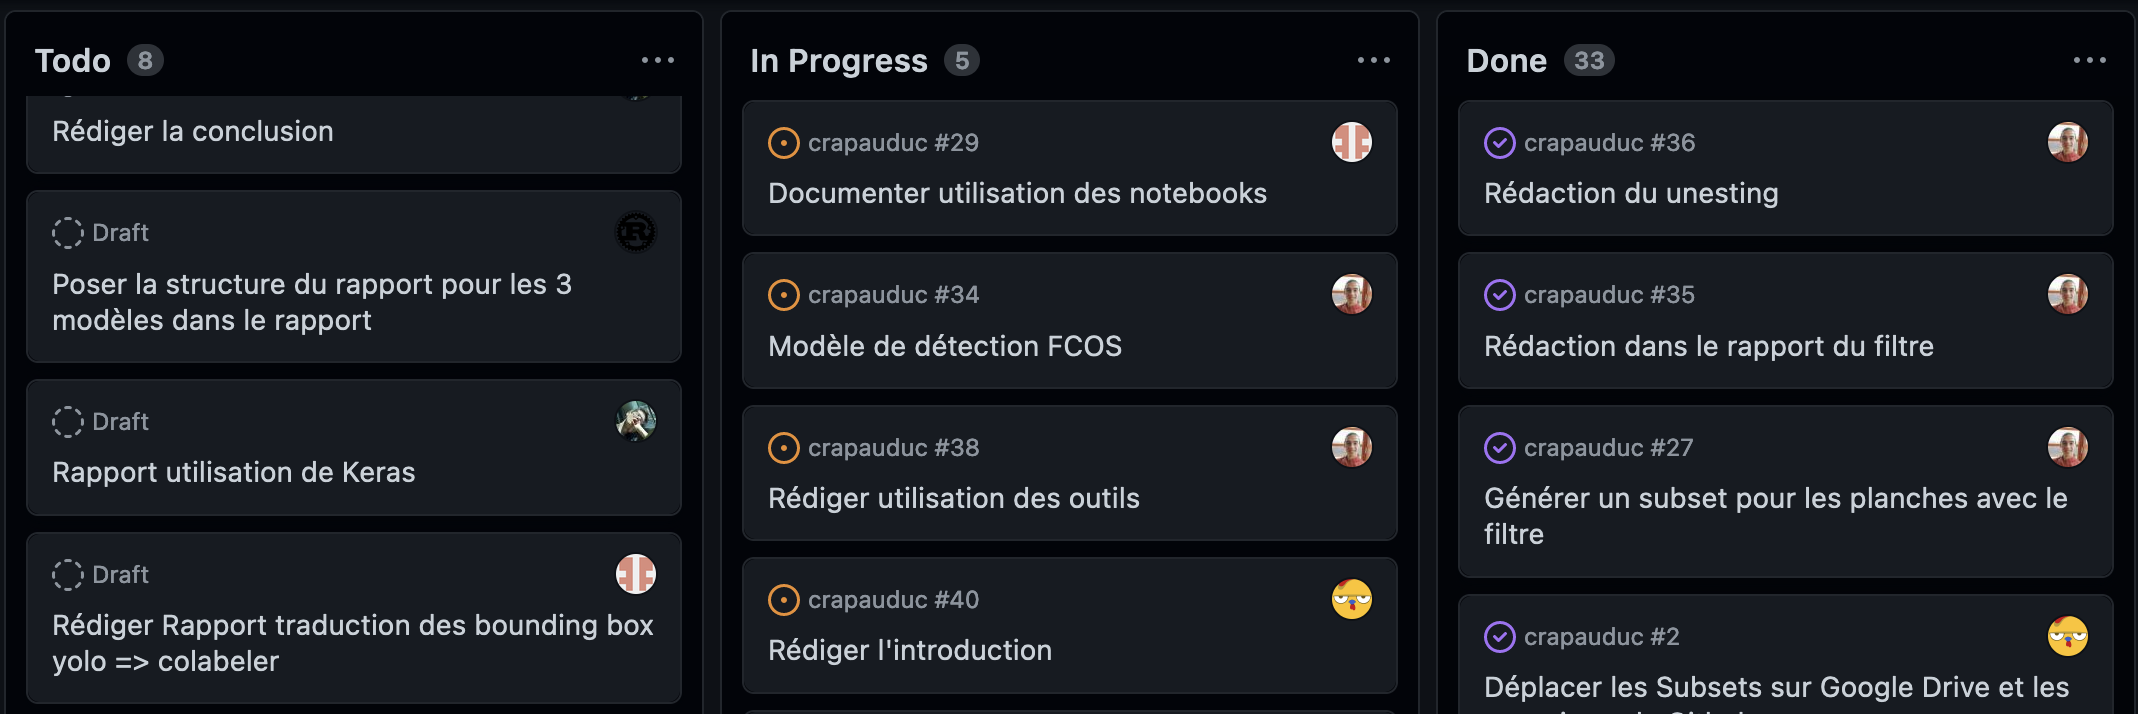
\includegraphics[width=0.8\linewidth]{images/kanban.png}
    \caption{Nos tâches du Kanban réparties en 3 catégories : à faire, en cours et terminées.}
    \label{fig:kanban}
\end{figure}

\paragraph{critique:} Nous avons décidé de ne pas élire de responsable au seins des étudiants. Cette décision a bien fonctionné pour certains aspects du travail, comme par exemple la prise des notes durant les réunions.
Cependant les appels Teams étaient généralement coordonés par Olivier et Joris sans vraiment que cela ait été prévu. Ce n'était pas voulu puisque nous souhaitions une organisation horizontale, mais cette manière de fonctionner s'est imposé naturellement et nous avons gardé cette organisation pour la suite. Par coordination nous entendons de manière générale animer la discussion et amorcer les points suivants. 
L'organisation de travail à elle aussi subit des changements au cours du projet. Au début, nous avons travaillé de manière très individuelle sur les petites tâches initiales. Nous souhaitions pouvoir travailler de manière très parallèle et ce choix semblait fut bon.
Néanmoins, cela nous a fait par la suite rencontrer deux nouveaux problèmes:
\begin{enumerate}
    \item Friction lors de la communication. \label{item:friction}
    \item Tâches trop complexes pour une seule personne. \label{item:complex}
\end{enumerate}
Notre organisation initiale fonctionnait bien au début du projet puisque nous avions beaucoup de petites tâches et nous avons bien avancé. 
Cependant, les tâches devenants de plus en plus grosses, les réunions ont pris de plus en plus de temps. 
En effet, nous avons rencontré beaucoup de problèmes qui étaient difficiles à résoudre seul, nous en discutions donc durant les réunions, et celles-ci commençait à prendre trop de temps.
Après quelques séances peu efficaces, nous avons réalisé qu'il serait plus judicieux de travail en petits groupes afin qu'une partie de la communication se fasse déjà entre les membres du sous-groupe et ainsi que l'on réduise les informations à partager lors des réunions. De plus travailler à plusieurs permettait de surmonter les problèmes rencontrés plus facilement.
\paragraph{}
Un second point que nous remarquons après ce travail et le suivant : nous avons souvent débloquer des problèmes en les abandonnant puis en y revenant plus tard, ceci nous a permis d'aborder le problème une seconde fois avec de nouvelles connaissances qui nous ont fait avoir une seconde approche différente.
\\
Avec notre organisation actuelle, c'est à dire une réunion par semaine, nous n'arrivions pas forcément bien à laisser quelques jour le problème pour y revenir à tête reposée. Nous pensons que faire des réunions moins régulièrement, toutes les deux semaines par exemple, permettrait d'avoir plus de temps et ainsi de retravailler plusieurs fois le même problème entre deux réunions. Cependant cette solution demande des membres du groupe une plus grande autonomie, néanmoins en alliant cette proposition avec les petits groupes de travail expliqué précédemment nous pensons que ça peut donner de bons résultats.

\paragraph{} En conclusion, nous sommes satisfait de l'organisation et du déroulement de ce projet, tous les membres du groupe ont travaillé sur des parties diverses et variées du projet. Tout le monde a ainsi pu expérimenter avec au moins un modèle de machine learning. De plus, la gestion s'est faite de manière naturelle et a permis de garder une bonne entente entre les différents étudiants même durant les moments où nous rencontrions des problèmes. Nous sommes particulièrement fière d'avoir su adapté notre organisation au cours du projet, afin de le mener à bien et ce malgrés notre manque de connaissance évident dans le domaine.